\documentclass[12pt]{beamer}
\usepackage{mypres}
\usepackage{etex}
\expandafter\def\expandafter\insertshorttitle\expandafter{%
  \insertshorttitle\hfill%
  \insertframenumber\,/\,\inserttotalframenumber}

\title[DeepPDE]{Forecasting Forces in Porosity Rock with Deep Neural Network}
\author{Aleksandr Katrutsa}
\institute[SkolTech]{Skolkovo Institute of Science and Technology\\
Moscow Institute of Physics and Techology     
}
\date{
    Moscow\\
    2015
}

\begin{document}

\maketitle

\begin{frame}{Plan}

\begin{enumerate}
\item Problem Statement
\item Data Generation
\item PDE solving
\item Deep Learning Application
\end{enumerate}

\end{frame}

\begin{frame}{Problem Statement}
Let $A$ be the covariance from the following family:
\[
A(x, y) = \exp\left(-\dfrac{\|x - y\|^2}{b^2}\right).
\]
The random field for the given covariance $k_A(x, y)$.

Consider PDE:
\[
{\rm div}(k_A(x, y) {\rm grad}(u(x, y))) = 1
\]
If solution $u(x, y)$ is known, one can compute the integral:
\[
f = \int\limits_{\Omega} u(x, y) dS
\]
The main goal is to find function $g$, which maps random field~$k_A(x, y)$ to the $f$ without direct solution of the PDE:
\[
g: k_A(x, y) \rightarrow f
\]

\end{frame}

\begin{frame}{Data Generation}
 
The goal of this stage is to generate random fields with given covariance $A$ fast.

The procedure:
\begin{itemize}
\item Compute decomposition $A = RR^{\top}$
\item Generate two random vectors $\mathbf{v}_1$ and $\mathbf{v}_2$ from $\mathcal{N}(0, I)$ and compose $\mathbf{v} = \mathbf{v}_1 + i\mathbf{v}_2$
\item Multiply $R\mathbf{v} = \mathbf{f}$, real and imaginary parts of $\mathbf{f}$ are independent random fields with given covariance $A$
\end{itemize}
\end{frame}

\begin{frame}{How to compute $A = RR^{\top}$ efficiently?}

\begin{itemize}
\item The covariance $A(x, y)$ is a symmetric Block Toeplitz with Toeplitz Block (BTTB) matrix $\Rightarrow$ to store it one needs only first column
\item Such matrix could be embedded to Block Circulant with Circulant Blocks (BCCB) matrix~$C$
\item BCCB matrix is diagonalized by 2D Fourier transform: 
\[
C = F^*\Lambda F
\]
\item $R = F^* \Lambda^{1/2} F$ 
\item Now matvec is really fast!
\end{itemize}

\end{frame}

\begin{frame}{Example}
\begin{center}
Random fields with different parameters $b^2$.
\end{center}

\begin{columns}
\column{0.5\textwidth}
\begin{figure}[!ht]
\centering
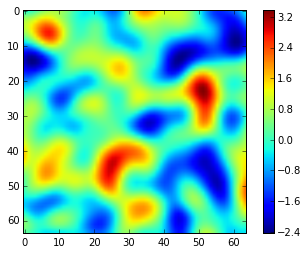
\includegraphics[width=0.8\textwidth]{rand_field1e-2.png}
\caption{$b^2 = 0.01$}
\end{figure}

\column{0.5\textwidth}
\begin{figure}[!ht]
\centering
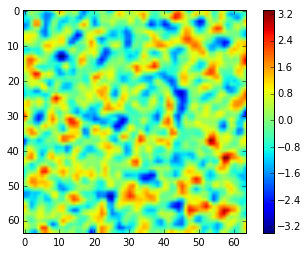
\includegraphics[width=0.8\textwidth]{rand_field1e-3.png}
\caption{$b^2 = 0.001$}
\end{figure}
\end{columns}
\end{frame}

\begin{frame}{Partial Differential Equation}
Consider partial differential equation:
\[
{\rm div}(k_A(x, y) {\rm grad}(u(x, y))) = 1,
\]
where $k_A(x, y)$ is the generated random field and $u(x, y)$ is unknown function.

Discretize domain with uniform mesh and convert continuous PDE to system of linear equation.
\end{frame}

\begin{frame}{Solution visualization}
\begin{center}
Parameter $b^2 = 0.01$.
\end{center}

\begin{columns}
\column{0.5\textwidth}
\begin{figure}[!ht]
\centering
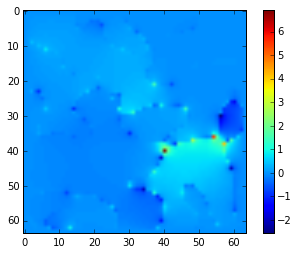
\includegraphics[width=0.8\textwidth]{sol1e-2.png}
\caption{Solution}
\end{figure}

\column{0.5\textwidth}
\begin{figure}[!ht]
\centering
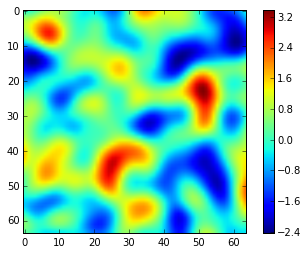
\includegraphics[width=0.8\textwidth]{rand_field1e-2.png}
\caption{Random field $k_A(x, y)$}
\end{figure}
\end{columns}

\end{frame}

\begin{frame}{Solution visualization}

\begin{center}
Parameter $b^2 = 0.001$.
\end{center}

\begin{columns}
\column{0.5\textwidth}
\begin{figure}[!ht]
\centering
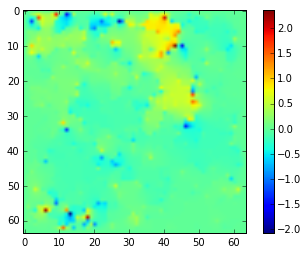
\includegraphics[width=0.8\textwidth]{sol1e-3.png}
\caption{Solution}
\end{figure}

\column{0.5\textwidth}
\begin{figure}[!ht]
\centering
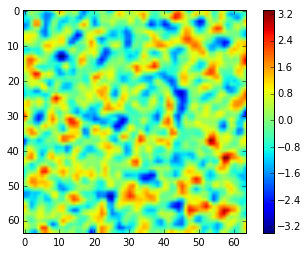
\includegraphics[width=0.8\textwidth]{rand_field1e-3.png}
\caption{Random field $k_A(x, y)$}
\end{figure}

\end{columns}

\end{frame}

\begin{frame}{Why Deep Neural Network?}
We want to find function $g$:
\[
g: k_A(x, y) \rightarrow f.
\]
Input: image of the random field

\begin{figure}[!ht]
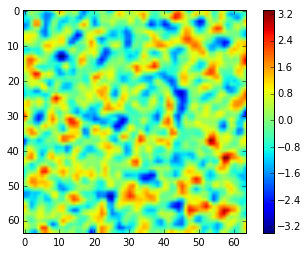
\includegraphics[scale=0.4]{rand_field1e-3.png}
\caption{Random field $k_A(x, y)$}
\end{figure}

Output: real number $f$
\end{frame}

\begin{frame}{Network Configuration}

\begin{equation*}
\begin{split}
& \text{Conv64-3} \rightarrow \text{Pool2} \rightarrow \text{FC100} \rightarrow \\ 
& \rightarrow \text{ReLU} \rightarrow \text{FC150} \rightarrow \text{ReLU} \rightarrow \text{Output}
\end{split}
\end{equation*}

Parameters: 
\begin{itemize}
\item number of epochs - 20\\
\item learning rate $= 0.01$, momentum $=0.9$
\end{itemize}
\end{frame}

\begin{frame}{Results}

\begin{figure}[!ht]
\centering
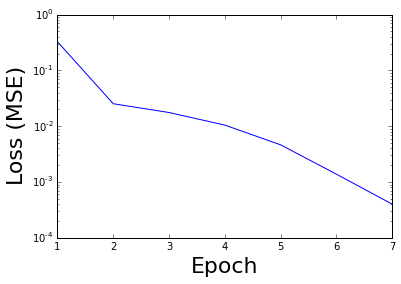
\includegraphics[scale=0.5]{convergence.png}
\caption{Convergence}
\end{figure}
\end{frame}

\begin{frame}
\begin{center}
\LARGE The End
\end{center}

\end{frame}

\end{document}
